\documentclass[11pt,
  english,
  a4paper,
]{article}
\usepackage{sa4ss}
\usepackage{amsmath,amssymb,array}
\usepackage{booktabs}

% From tagged-template.latex
\usepackage{lmodern}
\usepackage{ifxetex,ifluatex}
\ifnum 0\ifxetex 1\fi\ifluatex 1\fi=0 % if pdftex
  \usepackage[T1]{fontenc}
  \usepackage[utf8]{inputenc}
  \usepackage{textcomp} % provide euro and other symbols
\else % if luatex or xetex
  \usepackage{unicode-math}
  \defaultfontfeatures{Scale=MatchLowercase}
  \defaultfontfeatures[\rmfamily]{Ligatures=TeX,Scale=1}
\fi

% Use upquote if available, for straight quotes in verbatim environments
\IfFileExists{upquote.sty}{\usepackage{upquote}}{}
\IfFileExists{microtype.sty}{% use microtype if available
  \usepackage[]{microtype}
  \UseMicrotypeSet[protrusion]{basicmath} % disable protrusion for tt fonts
}{}
\makeatletter
\@ifundefined{KOMAClassName}{% if non-KOMA class
  \IfFileExists{parskip.sty}{%
    \usepackage{parskip}
  }{% else
    \setlength{\parindent}{0pt}
    \setlength{\parskip}{6pt plus 2pt minus 1pt}}
}{% if KOMA class
  \KOMAoptions{parskip=half}}
\makeatother
\usepackage{xcolor}
\IfFileExists{xurl.sty}{\usepackage{xurl}}{} % add URL line breaks if available
\hypersetup{
  pdftitle={Copper Rockfish (Sebastes caurinus) along the Washigton US West coast in 2020},
  pdflang={en},
  hidelinks,
  pdfcreator={LaTeX via pandoc}}
\urlstyle{same} % disable monospaced font for URLs
\usepackage{longtable}
% Correct order of tables after \paragraph or \subparagraph
\usepackage{etoolbox}
\makeatletter
\patchcmd\longtable{\par}{\if@noskipsec\mbox{}\fi\par}{}{}
\makeatother
% Allow footnotes in longtable head/foot
\IfFileExists{footnotehyper.sty}{\usepackage{footnotehyper}}{\usepackage{footnote}}
\makesavenoteenv{longtable}
\usepackage{graphicx}
\makeatletter
\def\maxwidth{\ifdim\Gin@nat@width>\linewidth\linewidth\else\Gin@nat@width\fi}
\def\maxheight{\ifdim\Gin@nat@height>\textheight\textheight\else\Gin@nat@height\fi}
\makeatother
% Scale images if necessary, so that they will not overflow the page
% margins by default, and it is still possible to overwrite the defaults
% using explicit options in \includegraphics[width, height, ...]{}
\setkeys{Gin}{width=\maxwidth,height=\maxheight,keepaspectratio}
% Set default figure placement to htbp
\makeatletter
\def\fps@figure{htbp}
\makeatother
\setlength{\emergencystretch}{3em} % prevent overfull lines
\providecommand{\tightlist}{%
  \setlength{\itemsep}{0pt}\setlength{\parskip}{0pt}}
\setcounter{secnumdepth}{5}
\ifxetex
  % Load polyglossia as late as possible: uses bidi with RTL langages (e.g. Hebrew, Arabic)
  \usepackage{polyglossia}
  \setmainlanguage[]{english}
\else
  \usepackage[shorthands=off,main=english]{babel}
\fi

\providecommand{\tightlist}{%
  \setlength{\itemsep}{0pt}\setlength{\parskip}{0pt}}


\date{}
\newcommand{\trTitle}{Copper Rockfish (\emph{Sebastes caurinus}) along the Washigton US West coast in 2020}
\newcommand{\trYear}{2020}
\newcommand{\trMonth}{December}
\newcommand{\trAuthsLong}{truetruetruetruetrue}
\newcommand{\trAuthsBack}{Wetzel, C.R., B.J. Langseth, J.M. Cope, T. Tsou, K.E. Hinton}
\newcommand{\trCitation}{
\begin{hangparas}{1em}{1}
\trAuthsBack{}. \trYear{}. \trTitle{}. Pacific Fisheries Management Council, Portland, Oregon. \pageref{LastPage}{}\,p.
\end{hangparas}}

\AtBeginDocument{\tagstructbegin{tag=Document}}
\AtEndDocument{\tagstructend}
\pretocmd{\maketitle}{\tagstructbegin{tag=H1}\tagmcbegin{tag=H1}}{}{}
\apptocmd{\maketitle}{\tagmcend\tagstructend}{}{}

\begin{document}

%%%%% Frontmatter %%%%%

% Footnote symbols in front matter
\renewcommand*{\thefootnote}{\fnsymbol{footnote}}

\small
\thispagestyle{empty}
\pagenumbering{roman}
\noindent
\begin{center}
\title{Copper Rockfish (\emph{Sebastes caurinus}) along the Washigton US West coast in 2020}
% \textnormal{\MakeTextUppercase{\trTitle{}}}
\vspace{1.5cm}
{\Large\textbf\newline{Copper Rockfish (\emph{Sebastes caurinus}) along the Washigton US West coast in 2020}}
\vfill
by\\
Chantel R. Wetzel\textsuperscript{1}\\
Brian J. Langseth\textsuperscript{1}\\
Jason M. Cope\textsuperscript{1}\\
Tien-Shui Tsou\textsuperscript{2}\\
Kristen E. Hinton\textsuperscript{2}\vfill
\textsuperscript{1}Northwest Fisheries Science Center, U.S. Department of Commerce, National Oceanic and Atmospheric Administration, National Marine Fisheries Service, 2725 Montlake Boulevard East, Seattle, Washington 98112\\
\textsuperscript{2}Washington Department of Fish and Wildlife, 600 Capital Way North, Olympia, Washington 98501\vfill
\trMonth{} \trYear{}
\end{center}
\clearpage

% Fourth page: Colophon
\thispagestyle{empty}
\vspace*{\fill}
\begin{center}
\copyright{} Pacific Fisheries Management Council, \trYear{}\\
\end{center}
\par
\bigskip
\noindent
Correct citation for this publication:
\bigskip
\par
\trCitation{}
\clearpage

% Add TOC to pdf bookmarks (clickable pdf)
\pdfbookmark[1]{\contentsname}{toc}

% Table of contents page, lists of figures and tables
\tableofcontents\clearpage
\listoffigures \listoftables \clearpage
\label{TRlastRoman}
\clearpage

% Table of contents
\newpage
\thispagestyle{empty} % to remove page number

% Settings for the main document
\pagenumbering{arabic}  % Regular page numbers
\pagestyle{plain}  % No page number on first page of main document, use 'empty'
\renewcommand*{\thefootnote}{\arabic{footnote}}  % Back to numeric footnotes
\setcounter{footnote}{0}  % And start at 1
\renewcommand{\headrulewidth}{0.5pt}
\renewcommand{\footrulewidth}{0.5pt}
%\pagestyle{fancy}\fancyhead[c]{Draft: Do not cite or circulate}

\newcommand{\lt}{\ensuremath <}
\newcommand{\gt}{\ensuremath >}

%Define cslreferences environment, required by pandoc 2.8
%https://github.com/rstudio/rmarkdown/issues/1649
\newlength{\cslhangindent}
\setlength{\cslhangindent}{1.5em}
\newenvironment{cslreferences}%
  {\setlength{\parindent}{0pt}%
  \everypar{\setlength{\hangindent}{\cslhangindent}}\ignorespaces}%
  {\par}

\pagebreak
\pagenumbering{roman}
\setcounter{page}{1}

\tagstructbegin{tag=H1}\tagmcbegin{tag=H1}

\hypertarget{executive-summary}{%
\section*{Executive Summary}\label{executive-summary}}
\addcontentsline{toc}{section}{Executive Summary}

\leavevmode\tagmcend\tagstructend

\tagstructbegin{tag=H2}\tagmcbegin{tag=H2}

\hypertarget{stock}{%
\subsection*{Stock}\label{stock}}
\addcontentsline{toc}{subsection}{Stock}

\leavevmode\tagmcend\tagstructend

\tagstructbegin{tag=P}\tagmcbegin{tag=P}

This assessment reports the status of Copper Rockfish (\emph{Sebastes caurinus}) off the US West coast using data through xxxx.

\leavevmode\tagmcend\tagstructend\par

\tagstructbegin{tag=P}\tagmcbegin{tag=P}

The years is 2020

\leavevmode\tagmcend\tagstructend\par

\tagstructbegin{tag=H2}\tagmcbegin{tag=H2}

\hypertarget{landings}{%
\subsection*{Landings}\label{landings}}
\addcontentsline{toc}{subsection}{Landings}

\leavevmode\tagmcend\tagstructend

\tagstructbegin{tag=P}\tagmcbegin{tag=P}

Replace text.

\leavevmode\tagmcend\tagstructend\par

\tagstructbegin{tag=P}\tagmcbegin{tag=P}

Table \ref{tab:ssb}.

\leavevmode\tagmcend\tagstructend\par

\begin{table}[H]

\caption{\label{tab:mortality}Removals by fleet for the last 10 years.}
\centering
\fontsize{10}{12}\selectfont
\fontsize{10}{12}\selectfont
\begin{tabular}[t]{r>{\centering\arraybackslash}p{2cm}>{\centering\arraybackslash}p{2cm}>{\centering\arraybackslash}p{2cm}}
\toprule
Year & Recreational (mt) & Commercial (mt) & Total Mortality\\
\midrule
2009 & 2732 & 0.00 & 2731.91\\
2010 & 2132 & 0.00 & 2132.14\\
2011 & 2642 & 0.00 & 2641.62\\
2012 & 1760 & 0.00 & 1759.56\\
2013 & 2562 & 0.00 & 2561.77\\
2014 & 2343 & 0.00 & 2343.20\\
2015 & 1319 & 0.00 & 1318.84\\
2016 & 1854 & 0.00 & 1853.86\\
2017 & 1294 & 0.01 & 1293.99\\
2018 & 3025 & 0.00 & 3024.60\\
2019 & 4274 & 0.00 & 4273.52\\
2020 & 0 & 0.00 & 0.00\\
\bottomrule
\end{tabular}
\end{table}

\tagstructbegin{tag=P}\tagmcbegin{tag=P}

Here is a reference to the catches (Table \ref{tab:mortality})

\leavevmode\tagmcend\tagstructend\par

\tagstructbegin{tag=H2}\tagmcbegin{tag=H2}

\hypertarget{data-and-assessment}{%
\subsection*{Data and Assessment}\label{data-and-assessment}}
\addcontentsline{toc}{subsection}{Data and Assessment}

\leavevmode\tagmcend\tagstructend

\tagstructbegin{tag=P}\tagmcbegin{tag=P}

Replace text.

\leavevmode\tagmcend\tagstructend\par

\tagstructbegin{tag=H2}\tagmcbegin{tag=H2}

\hypertarget{stock-biomass}{%
\subsection*{Stock Biomass}\label{stock-biomass}}
\addcontentsline{toc}{subsection}{Stock Biomass}

\leavevmode\tagmcend\tagstructend

\tagstructbegin{tag=P}\tagmcbegin{tag=P}

Replace text.

\leavevmode\tagmcend\tagstructend\par

\begin{table}[H]

\caption{\label{tab:ssb}Estimated spawning output and the fraction unfished and the 95 percent confidence intervals.}
\centering
\fontsize{10}{12}\selectfont
\fontsize{10}{12}\selectfont
\begin{tabular}[t]{r>{\centering\arraybackslash}p{1.57cm}>{\centering\arraybackslash}p{1.57cm}>{\centering\arraybackslash}p{1.57cm}>{\centering\arraybackslash}p{1.57cm}>{\centering\arraybackslash}p{1.57cm}>{\centering\arraybackslash}p{1.57cm}}
\toprule
Year & Spawning Output & Lower Interval & Upper Interval & Fraction Unfished & Lower Interval & Upper Interval\\
\midrule
2009 & 3786 & 3786 & 3786 & 0.451 & 0.451 & 0.451\\
2010 & 3738 & 3738 & 3738 & 0.445 & 0.445 & 0.445\\
2011 & 3756 & 3756 & 3756 & 0.447 & 0.447 & 0.447\\
2012 & 3726 & 3726 & 3726 & 0.444 & 0.444 & 0.444\\
2013 & 3786 & 3786 & 3786 & 0.451 & 0.451 & 0.451\\
2014 & 3766 & 3766 & 3766 & 0.449 & 0.449 & 0.449\\
2015 & 3767 & 3767 & 3767 & 0.449 & 0.449 & 0.449\\
2016 & 3872 & 3872 & 3872 & 0.461 & 0.461 & 0.461\\
2017 & 3922 & 3922 & 3922 & 0.467 & 0.467 & 0.467\\
2018 & 4029 & 4029 & 4029 & 0.480 & 0.480 & 0.480\\
2019 & 3956 & 3956 & 3956 & 0.471 & 0.471 & 0.471\\
2020 & 3750 & 3750 & 3750 & 0.447 & 0.447 & 0.447\\
2021 & 3979 & 3979 & 3979 & 0.474 & 0.474 & 0.474\\
\bottomrule
\end{tabular}
\end{table}

\tagstructbegin{tag=H2}\tagmcbegin{tag=H2}

\hypertarget{recruitment}{%
\subsection*{Recruitment}\label{recruitment}}
\addcontentsline{toc}{subsection}{Recruitment}

\leavevmode\tagmcend\tagstructend

\tagstructbegin{tag=P}\tagmcbegin{tag=P}

Replace text.

\leavevmode\tagmcend\tagstructend\par

\begin{table}[H]

\caption{\label{tab:recr}Estimated recruitment and recruitment deviations (recruit devs.) and the 95 percent confidence intervals.}
\centering
\fontsize{10}{12}\selectfont
\fontsize{10}{12}\selectfont
\begin{tabular}[t]{r>{\centering\arraybackslash}p{1.57cm}>{\centering\arraybackslash}p{1.57cm}>{\centering\arraybackslash}p{1.57cm}>{\centering\arraybackslash}p{1.57cm}>{\centering\arraybackslash}p{1.57cm}>{\centering\arraybackslash}p{1.57cm}}
\toprule
Year & Recruitment & Lower Interval & Upper Interval & Recruit Devs. & Lower Interval & Upper Interval\\
\midrule
2009 & 7760 & 7760 & 7760 & 0 & 0 & 0\\
2010 & 7741 & 7741 & 7741 & 0 & 0 & 0\\
2011 & 7748 & 7748 & 7748 & 0 & 0 & 0\\
2012 & 7736 & 7736 & 7736 & 0 & 0 & 0\\
2013 & 7760 & 7760 & 7760 & 0 & 0 & 0\\
2014 & 7752 & 7752 & 7752 & 0 & 0 & 0\\
2015 & 7753 & 7753 & 7753 & 0 & 0 & 0\\
2016 & 7793 & 7793 & 7793 & 0 & 0 & 0\\
2017 & 7812 & 7812 & 7812 & 0 & 0 & 0\\
2018 & 7851 & 7851 & 7851 & 0 & 0 & 0\\
2019 & 7825 & 7825 & 7825 & 0 & 0 & 0\\
2020 & 7746 & 7746 & 7746 & 0 & 0 & 0\\
2021 & 7833 & 7833 & 7833 & 0 & 0 & 0\\
\bottomrule
\end{tabular}
\end{table}

\tagstructbegin{tag=H2}\tagmcbegin{tag=H2}

\hypertarget{exploitation-status}{%
\subsection*{Exploitation Status}\label{exploitation-status}}
\addcontentsline{toc}{subsection}{Exploitation Status}

\leavevmode\tagmcend\tagstructend

\tagstructbegin{tag=P}\tagmcbegin{tag=P}

Replace text.

\leavevmode\tagmcend\tagstructend\par

\begin{table}[H]

\caption{\label{tab:expliot}Estimated 1-SPR in percent and the exploitation rate (Exploit. Rate) and the 95 percent confidence intervals.}
\centering
\fontsize{10}{12}\selectfont
\fontsize{10}{12}\selectfont
\begin{tabular}[t]{r>{\centering\arraybackslash}p{1.57cm}>{\centering\arraybackslash}p{1.57cm}>{\centering\arraybackslash}p{1.57cm}>{\centering\arraybackslash}p{1.57cm}>{\centering\arraybackslash}p{1.57cm}>{\centering\arraybackslash}p{1.57cm}}
\toprule
Year & 1-SPR & Lower Interval & Upper Interval & Exploit. Rate & Lower Interval & Upper Interval\\
\midrule
2009 & 54.5 & 54.5 & 54.5 & 0.067 & 0.067 & 0.067\\
2010 & 47.5 & 47.5 & 47.5 & 0.053 & 0.053 & 0.053\\
2011 & 53.6 & 53.6 & 53.6 & 0.065 & 0.065 & 0.065\\
2012 & 42.0 & 42.0 & 42.0 & 0.043 & 0.043 & 0.043\\
2013 & 52.4 & 52.4 & 52.4 & 0.062 & 0.062 & 0.062\\
2014 & 49.9 & 49.9 & 49.9 & 0.057 & 0.057 & 0.057\\
2015 & 34.1 & 34.1 & 34.1 & 0.032 & 0.032 & 0.032\\
2016 & 42.5 & 42.5 & 42.5 & 0.044 & 0.044 & 0.044\\
2017 & 32.8 & 32.8 & 32.8 & 0.031 & 0.031 & 0.031\\
2018 & 55.7 & 55.7 & 55.7 & 0.070 & 0.070 & 0.070\\
2019 & 66.5 & 66.5 & 66.5 & 0.101 & 0.101 & 0.101\\
2020 & 0.0 & 0.0 & 0.0 & 0.000 & 0.000 & 0.000\\
\bottomrule
\end{tabular}
\end{table}

\tagstructbegin{tag=H2}\tagmcbegin{tag=H2}

\hypertarget{reference-points}{%
\subsection*{Reference Points}\label{reference-points}}
\addcontentsline{toc}{subsection}{Reference Points}

\leavevmode\tagmcend\tagstructend

\tagstructbegin{tag=P}\tagmcbegin{tag=P}

Replace text.

\leavevmode\tagmcend\tagstructend\par

\begin{table}[H]

\caption{\label{tab:ref}Reference points}
\centering
\fontsize{10}{12}\selectfont
\fontsize{10}{12}\selectfont
\begin{tabular}[t]{>{\raggedleft\arraybackslash}p{6cm}>{\raggedleft\arraybackslash}p{2cm}>{\raggedleft\arraybackslash}p{2cm}c}
\toprule
Metric & Estimate & Lower Inteval & Upper Interval\\
\midrule
Unfished Spawning Output & 8395.78 & 8395.78 & 8395.78\\
Unfished Age 3+ Biomass (mt) & 80028.40 & 80028.40 & 80028.40\\
Unfished Recruitment (R0) & 8678.67 & 8678.67 & 8678.67\\
Spawning Output (2021) & 3978.78 & 3978.78 & 3978.78\\
Fraction Unfished (2021) & 0.47 & 0.47 & 0.47\\
Reference Points Based SB40 Percent & NA & NA & NA\\
Proxy Spawning Output(SB40 Percent & 3358.31 & 3358.31 & 3358.31\\
SPR Resulting in SB40 Percent & 0.46 & 0.46 & 0.46\\
Exploitation Rate Resulting in SB40 Percent & 0.07 & 0.07 & 0.07\\
Yield with SPR Based On SB40 Percent (mt) & 2451.87 & 2451.87 & 2451.87\\
Reference Points Based on SPR Proxy for MSY & NA & NA & NA\\
Proxy Spawning Output (SPR50) & 3745.81 & 3745.81 & 3745.81\\
SPR50 & 50.00 & NA & NA\\
Exploitation Rate Corresponding to SPR50 & 0.06 & 0.06 & 0.06\\
Yield with SPR50 at SB SPR (mt) & 2336.95 & 2336.95 & 2336.95\\
Reference Points Based on Estimated MSY Values & NA & NA & NA\\
Spawning Output at MSY (SB MSY) & 2259.48 & 2259.48 & 2259.48\\
SPR MSY & 0.34 & 0.34 & 0.34\\
Exploitation Rate Corresponding to SPR MSY & 0.10 & 0.10 & 0.10\\
MSY (mt) & 2616.45 & 2616.45 & 2616.45\\
\bottomrule
\end{tabular}
\end{table}

\tagstructbegin{tag=H2}\tagmcbegin{tag=H2}

\hypertarget{management-performance}{%
\subsection*{Management Performance}\label{management-performance}}
\addcontentsline{toc}{subsection}{Management Performance}

\leavevmode\tagmcend\tagstructend

\tagstructbegin{tag=P}\tagmcbegin{tag=P}

Replace text.

\leavevmode\tagmcend\tagstructend\par

\begin{table}[H]

\caption{\label{tab:manage}The OFL, ABC, ACL, and Landings for the last 10 years.}
\centering
\fontsize{10}{12}\selectfont
\fontsize{10}{12}\selectfont
\begin{tabular}[t]{r>{\centering\arraybackslash}p{2.2cm}>{\centering\arraybackslash}p{2.2cm}>{\centering\arraybackslash}p{2.2cm}>{\centering\arraybackslash}p{2.2cm}}
\toprule
Years & OFL & ABC & ACL & Landings\\
\midrule
2009 & fill in & fill in & fill in & 2,731.91\\
2010 & fill in & fill in & fill in & 2,132.14\\
2011 & fill in & fill in & fill in & 2,641.62\\
2012 & fill in & fill in & fill in & 1,759.56\\
2013 & fill in & fill in & fill in & 2,561.77\\
2014 & fill in & fill in & fill in & 2,343.20\\
2015 & fill in & fill in & fill in & 1,318.84\\
2016 & fill in & fill in & fill in & 1,853.86\\
2017 & fill in & fill in & fill in & 1,293.99\\
2018 & fill in & fill in & fill in & 3,024.60\\
2019 & fill in & fill in & fill in & 4,273.52\\
2020 & fill in & fill in & fill in & 0.00\\
\bottomrule
\end{tabular}
\end{table}

\tagstructbegin{tag=H2}\tagmcbegin{tag=H2}

\hypertarget{unresolved-problems-and-major-uncertainties}{%
\subsection*{Unresolved Problems and Major Uncertainties}\label{unresolved-problems-and-major-uncertainties}}
\addcontentsline{toc}{subsection}{Unresolved Problems and Major Uncertainties}

\leavevmode\tagmcend\tagstructend

\tagstructbegin{tag=P}\tagmcbegin{tag=P}

Replace text.

\leavevmode\tagmcend\tagstructend\par

\tagstructbegin{tag=H2}\tagmcbegin{tag=H2}

\hypertarget{decision-table}{%
\subsection*{Decision Table}\label{decision-table}}
\addcontentsline{toc}{subsection}{Decision Table}

\leavevmode\tagmcend\tagstructend

\tagstructbegin{tag=P}\tagmcbegin{tag=P}

Add the projection table

\leavevmode\tagmcend\tagstructend\par

\begin{table}[H]

\caption{\label{tab:project}Projections}
\centering
\fontsize{10}{12}\selectfont
\fontsize{10}{12}\selectfont
\begin{tabular}[t]{r>{\centering\arraybackslash}p{1.83cm}>{\centering\arraybackslash}p{1.83cm}>{\centering\arraybackslash}p{1.83cm}>{\centering\arraybackslash}p{1.83cm}>{\centering\arraybackslash}p{1.83cm}}
\toprule
Year & OFL & ABC & 3+ Biomass & Spawning Output & Fraction Unfished\\
\midrule
2021 & 2464.1 & 60.1 & 42774.5 & 3978.8 & 0.474\\
2022 & 2595.7 & 60.4 & 44920.2 & 4208.4 & 0.501\\
2023 & 2724.0 & 2724.0 & 46987.6 & 4440.5 & 0.529\\
2024 & 2688.4 & 2688.4 & 46401.4 & 4394.1 & 0.523\\
2025 & 2651.9 & 2651.9 & 45839.6 & 4341.6 & 0.517\\
2026 & 2617.4 & 2617.4 & 45324.6 & 4286.0 & 0.510\\
2027 & 2586.6 & 2586.6 & 44855.2 & 4231.5 & 0.504\\
2028 & 2559.8 & 2559.8 & 44433.3 & 4181.2 & 0.498\\
2029 & 2536.5 & 2536.5 & 44056.3 & 4136.3 & 0.493\\
2030 & 2516.3 & 2516.3 & 43720.3 & 4096.7 & 0.488\\
2031 & 2498.6 & 2498.6 & 43420.5 & 4061.8 & 0.484\\
2032 & 2482.9 & 2482.9 & 43152.7 & 4030.8 & 0.480\\
\bottomrule
\end{tabular}
\end{table}

\tagstructbegin{tag=P}\tagmcbegin{tag=P}

Replace text.

\leavevmode\tagmcend\tagstructend\par

\tagstructbegin{tag=H2}\tagmcbegin{tag=H2}

\hypertarget{research-and-data-needs}{%
\subsection*{Research and Data Needs}\label{research-and-data-needs}}
\addcontentsline{toc}{subsection}{Research and Data Needs}

\leavevmode\tagmcend\tagstructend

\tagstructbegin{tag=P}\tagmcbegin{tag=P}

Replace text.

\leavevmode\tagmcend\tagstructend\par

\pagebreak
\setlength{\parskip}{5mm plus1mm minus1mm}
\pagenumbering{arabic}
\setcounter{page}{1}
\renewcommand{\thefigure}{\arabic{figure}}
\renewcommand{\thetable}{\arabic{table}}

\tagstructbegin{tag=H1}\tagmcbegin{tag=H1}

\hypertarget{introduction}{%
\section{Introduction}\label{introduction}}

\leavevmode\tagmcend\tagstructend

\tagstructbegin{tag=H2}\tagmcbegin{tag=H2}

\hypertarget{basic-information}{%
\subsection{Basic Information}\label{basic-information}}

\leavevmode\tagmcend\tagstructend

\tagstructbegin{tag=P}\tagmcbegin{tag=P}

This assessment reports the status of Copper Rockfish (\emph{Sebastes caurinus}) off the US West coast using data through xxxx.

\leavevmode\tagmcend\tagstructend\par

\tagstructbegin{tag=H2}\tagmcbegin{tag=H2}

\hypertarget{life-history}{%
\subsection{Life History}\label{life-history}}

\leavevmode\tagmcend\tagstructend

\tagstructbegin{tag=P}\tagmcbegin{tag=P}

Replace text.

\leavevmode\tagmcend\tagstructend\par

\tagstructbegin{tag=H2}\tagmcbegin{tag=H2}

\hypertarget{ecosystem-considerations}{%
\subsection{Ecosystem Considerations}\label{ecosystem-considerations}}

\leavevmode\tagmcend\tagstructend

\tagstructbegin{tag=P}\tagmcbegin{tag=P}

Replace text.

\leavevmode\tagmcend\tagstructend\par

\tagstructbegin{tag=H2}\tagmcbegin{tag=H2}

\hypertarget{historical-and-current-fishery-information}{%
\subsection{Historical and Current Fishery Information}\label{historical-and-current-fishery-information}}

\leavevmode\tagmcend\tagstructend

\tagstructbegin{tag=P}\tagmcbegin{tag=P}

Replace text.

\leavevmode\tagmcend\tagstructend\par

\tagstructbegin{tag=H2}\tagmcbegin{tag=H2}

\hypertarget{summary-of-management-history-and-performance}{%
\subsection{Summary of Management History and Performance}\label{summary-of-management-history-and-performance}}

\leavevmode\tagmcend\tagstructend

\tagstructbegin{tag=P}\tagmcbegin{tag=P}

Replace text.

\leavevmode\tagmcend\tagstructend\par

\tagstructbegin{tag=H2}\tagmcbegin{tag=H2}

\hypertarget{foreign-fisheries}{%
\subsection{Foreign Fisheries}\label{foreign-fisheries}}

\leavevmode\tagmcend\tagstructend

\tagstructbegin{tag=P}\tagmcbegin{tag=P}

Replace text.

\leavevmode\tagmcend\tagstructend\par

\tagstructbegin{tag=H1}\tagmcbegin{tag=H1}

\hypertarget{data}{%
\section{Data}\label{data}}

\leavevmode\tagmcend\tagstructend

\tagstructbegin{tag=P}\tagmcbegin{tag=P}

A description of each data source is provided below (Figure \ref{fig:data-plot}).

\leavevmode\tagmcend\tagstructend\par

\tagstructbegin{tag=H2}\tagmcbegin{tag=H2}

\hypertarget{fishery-dependent-data}{%
\subsection{Fishery-Dependent Data}\label{fishery-dependent-data}}

\leavevmode\tagmcend\tagstructend

\tagstructbegin{tag=H2}\tagmcbegin{tag=H2}

\hypertarget{fishery-independent-data}{%
\subsection{Fishery-Independent Data}\label{fishery-independent-data}}

\leavevmode\tagmcend\tagstructend

\tagstructbegin{tag=H3}\tagmcbegin{tag=H3}

\hypertarget{nwfsc-slope}{%
\subsubsection{NWFSC Slope}\label{nwfsc-slope}}

\leavevmode\tagmcend\tagstructend

\tagstructbegin{tag=H3}\tagmcbegin{tag=H3}

\hypertarget{section}{%
\subsubsection{\texorpdfstring{\acrlong{s-tri}}{}}\label{section}}

\leavevmode\tagmcend\tagstructend

\tagstructbegin{tag=P}\tagmcbegin{tag=P}

The \gls{s-tri} was first conducted by the \gls{afsc} in 1977, and the survey continued until 2004 {\tagstructbegin{tag=Reference}\tagmcbegin{tag=Reference}(Weinberg et al. 2002)\leavevmode\tagmcend\tagstructend}. Its basic design was a series of equally-spaced east-to-west transects across the continential shelf from which searches for tows in a specific depth range were initiated. The survey design changed slightly over time. In general, all of the surveys were conducted in the mid summer through early fall. The 1977 survey was conducted from early July through late September. The surveys from 1980 through 1989 were conducted from mid-July to late September. The 1992 survey was conducted from mid July through early October. The 1995 survey was conducted from early June through late August. The 1998 survey was conducted from early June through early August. Finally, the 2001 and 2004 surveys were conducted from May to July.

\leavevmode\tagmcend\tagstructend\par

\tagstructbegin{tag=P}\tagmcbegin{tag=P}

Haul depths ranged from 91-457 m during the 1977 survey with no hauls shallower than 91 m. Due to haul performance issues and truncated sampling with respect to depth, the data from 1977 were omitted from this analysis. The surveys in 1980, 1983, and 1986 covered the US West Coast south to 36.8\textdegree N latitude and a depth range of 55-366 m. The surveys in 1989 and 1992 covered the same depth range but extended the southern range to 34.5\textdegree N (near Point Conception). From 1995 through 2004, the surveys covered the depth range 55-500 m and surveyed south to 34.5\textdegree N. In 2004, the final year of the \gls{s-tri} series, the \gls{nwfsc} \gls{fram} conducted the survey following similar protocols to earlier years.

\leavevmode\tagmcend\tagstructend\par

\tagstructbegin{tag=H3}\tagmcbegin{tag=H3}

\hypertarget{nwfsc-slope-1}{%
\subsubsection{NWFSC Slope}\label{nwfsc-slope-1}}

\leavevmode\tagmcend\tagstructend

\tagstructbegin{tag=H3}\tagmcbegin{tag=H3}

\hypertarget{section-1}{%
\subsubsection{\texorpdfstring{\acrlong{s-wcgbt}}{}}\label{section-1}}

\leavevmode\tagmcend\tagstructend

\tagstructbegin{tag=P}\tagmcbegin{tag=P}

The \Gls{s-wcgbt} is based on a random-grid design; covering the coastal waters from a depth of 55-1,280 m {\tagstructbegin{tag=Reference}\tagmcbegin{tag=Reference}(Bradburn, Keller, and Horness 2011)\leavevmode\tagmcend\tagstructend}. This design generally uses four industry-chartered vessels per year assigned to a roughly equal number of randomly selected grid cells and divided into two `passes' of the coast. Two vessels fish from north to south during each pass between late May to early October. This design therefore incorporates both vessel-to-vessel differences in catchability, as well as variance associated with selecting a relatively small number (approximately 700) of possible cells from a very large set of possible cells spread from the Mexican to the Canadian borders.

\leavevmode\tagmcend\tagstructend\par

\tagstructbegin{tag=H2}\tagmcbegin{tag=H2}

\hypertarget{biological-data}{%
\subsection{Biological Data}\label{biological-data}}

\leavevmode\tagmcend\tagstructend

\tagstructbegin{tag=H3}\tagmcbegin{tag=H3}

\hypertarget{natural-mortality}{%
\subsubsection{Natural Mortality}\label{natural-mortality}}

\leavevmode\tagmcend\tagstructend

\tagstructbegin{tag=P}\tagmcbegin{tag=P}

Hamel {\tagstructbegin{tag=Reference}\tagmcbegin{tag=Reference}(2015)\leavevmode\tagmcend\tagstructend} developed a method for combining meta-analytic approaches relating the {\tagstructbegin{tag=Formula}\tagmcbegin{tag=Formula}\(M\)\leavevmode\tagmcend\tagstructend} rate to other life-history parameters such as longevity, size, growth rate, and reproductive effort to provide a prior on {\tagstructbegin{tag=Formula}\tagmcbegin{tag=Formula}\(M\)\leavevmode\tagmcend\tagstructend}. In that same issue of \emph{ICES Journal of Marine Science}, Then et al.~(XXX) provided an updated data set of estimates of {\tagstructbegin{tag=Formula}\tagmcbegin{tag=Formula}\(M\)\leavevmode\tagmcend\tagstructend} and related life history parameters across a large number of fish species from which to develop an {\tagstructbegin{tag=Formula}\tagmcbegin{tag=Formula}\(M\)\leavevmode\tagmcend\tagstructend} estimator for fish species in general. They concluded by recommending {\tagstructbegin{tag=Formula}\tagmcbegin{tag=Formula}\(M\)\leavevmode\tagmcend\tagstructend} estimates be based on maximum age alone, based on an updated Hoenig non-linear least squares estimator {\tagstructbegin{tag=Formula}\tagmcbegin{tag=Formula}\(M=4.899A^{-0.916}_{max}\)\leavevmode\tagmcend\tagstructend}. The approach of basing {\tagstructbegin{tag=Formula}\tagmcbegin{tag=Formula}\(M\)\leavevmode\tagmcend\tagstructend} priors on maximum age alone was one that was already being used for West Coast rockfish assessments. However, in fitting the alternative model forms relating {\tagstructbegin{tag=Formula}\tagmcbegin{tag=Formula}\(M\)\leavevmode\tagmcend\tagstructend} to {\tagstructbegin{tag=Formula}\tagmcbegin{tag=Formula}\(A_{\text{max}}\)\leavevmode\tagmcend\tagstructend}, Then et al.~(XXX) did not consistently apply their transformation. In particular, in real space, one would expect substantial heteroscedasticity in both the observation and process error associated with the observed relationship of {\tagstructbegin{tag=Formula}\tagmcbegin{tag=Formula}\(M\)\leavevmode\tagmcend\tagstructend} to {\tagstructbegin{tag=Formula}\tagmcbegin{tag=Formula}\(A_{\text{max}}\)\leavevmode\tagmcend\tagstructend}. Therefore, it would be reasonable to fit all models under a log transformation. This was not done. Re-evaluating the data used in Then et al.~(XXX) by fitting the one-parameter {\tagstructbegin{tag=Formula}\tagmcbegin{tag=Formula}\(A_{\text{max}}\)\leavevmode\tagmcend\tagstructend} model under a log-log transformation (such that the slope is forced to be -1 in the transformed space Hamel XXX), the point estimate for {\tagstructbegin{tag=Formula}\tagmcbegin{tag=Formula}\(M\)\leavevmode\tagmcend\tagstructend} is:

\leavevmode\tagmcend\tagstructend\par

\begin{centering}

$M=\frac{5.4}{A_{\text{max}}}$

\end{centering}

\tagstructbegin{tag=P}\tagmcbegin{tag=P}

The above is also the median of the prior. The prior is defined as a lognormal distribution with mean {\tagstructbegin{tag=Formula}\tagmcbegin{tag=Formula}\(ln(5.4/A_{\text{max}})\)\leavevmode\tagmcend\tagstructend} and SE = 0.438. Using a maximum age of 50, the point estimate and median of the prior is 0.108 per year The maximum age was selected based on available age data from all West Coast data sources. The oldest aged rockfish was XXX years, captured off the coast of XXX in XXX. However, age data are subject to ageing error which could impact this estimate of longevity. The selection of 50 years was based on the range of other ages available with multiple observations of fish between XXX and XXX years of age and literature examining the longevity of \texttt{spp}.

\leavevmode\tagmcend\tagstructend\par

\tagstructbegin{tag=H3}\tagmcbegin{tag=H3}

\hypertarget{maturation-and-fecundity}{%
\subsubsection{Maturation and Fecundity}\label{maturation-and-fecundity}}

\leavevmode\tagmcend\tagstructend

\tagstructbegin{tag=H3}\tagmcbegin{tag=H3}

\hypertarget{sex-ratio}{%
\subsubsection{Sex Ratio}\label{sex-ratio}}

\leavevmode\tagmcend\tagstructend

\tagstructbegin{tag=H3}\tagmcbegin{tag=H3}

\hypertarget{length-weight-relationship}{%
\subsubsection{Length-Weight Relationship}\label{length-weight-relationship}}

\leavevmode\tagmcend\tagstructend

\tagstructbegin{tag=H3}\tagmcbegin{tag=H3}

\hypertarget{growth-length-at-age}{%
\subsubsection{Growth (Length-at-Age)}\label{growth-length-at-age}}

\leavevmode\tagmcend\tagstructend

\tagstructbegin{tag=H3}\tagmcbegin{tag=H3}

\hypertarget{ageing-precision-and-bias}{%
\subsubsection{Ageing Precision and Bias}\label{ageing-precision-and-bias}}

\leavevmode\tagmcend\tagstructend

\tagstructbegin{tag=H2}\tagmcbegin{tag=H2}

\hypertarget{environmental-and-ecosystem-data}{%
\subsection{Environmental and Ecosystem Data}\label{environmental-and-ecosystem-data}}

\leavevmode\tagmcend\tagstructend

\tagstructbegin{tag=H1}\tagmcbegin{tag=H1}

\hypertarget{assessment-model}{%
\section{Assessment Model}\label{assessment-model}}

\leavevmode\tagmcend\tagstructend

\tagstructbegin{tag=H2}\tagmcbegin{tag=H2}

\hypertarget{summary-of-previous-assessments-and-reviews}{%
\subsection{Summary of Previous Assessments and Reviews}\label{summary-of-previous-assessments-and-reviews}}

\leavevmode\tagmcend\tagstructend

\tagstructbegin{tag=H3}\tagmcbegin{tag=H3}

\hypertarget{history-of-modeling-approaches-not-required-for-an-update-assessment}{%
\subsubsection{History of Modeling Approaches (not required for an update assessment)}\label{history-of-modeling-approaches-not-required-for-an-update-assessment}}

\leavevmode\tagmcend\tagstructend

\tagstructbegin{tag=H3}\tagmcbegin{tag=H3}

\hypertarget{most-recent-star-panel-and-ssc-recommendations-not-required-for-an-update-assessment}{%
\subsubsection{Most Recent STAR Panel and SSC Recommendations (not required for an update assessment)}\label{most-recent-star-panel-and-ssc-recommendations-not-required-for-an-update-assessment}}

\leavevmode\tagmcend\tagstructend

\tagstructbegin{tag=H3}\tagmcbegin{tag=H3}

\hypertarget{response-to-groundfish-subcommittee-requests-not-required-in-draft}{%
\subsubsection{Response to Groundfish Subcommittee Requests (not required in draft)}\label{response-to-groundfish-subcommittee-requests-not-required-in-draft}}

\leavevmode\tagmcend\tagstructend

\tagstructbegin{tag=H2}\tagmcbegin{tag=H2}

\hypertarget{model-structure-and-assumptions}{%
\subsection{Model Structure and Assumptions}\label{model-structure-and-assumptions}}

\leavevmode\tagmcend\tagstructend

\tagstructbegin{tag=H3}\tagmcbegin{tag=H3}

\hypertarget{model-changes-from-the-last-assessment-not-required-for-an-update-assessment}{%
\subsubsection{Model Changes from the Last Assessment (not required for an update assessment)}\label{model-changes-from-the-last-assessment-not-required-for-an-update-assessment}}

\leavevmode\tagmcend\tagstructend

\tagstructbegin{tag=H3}\tagmcbegin{tag=H3}

\hypertarget{modeling-platform-and-structure}{%
\subsubsection{Modeling Platform and Structure}\label{modeling-platform-and-structure}}

\leavevmode\tagmcend\tagstructend

\tagstructbegin{tag=P}\tagmcbegin{tag=P}

General model specifications (e.g., executable version, model structure, definition of fleets and areas)

\leavevmode\tagmcend\tagstructend\par

\tagstructbegin{tag=H3}\tagmcbegin{tag=H3}

\hypertarget{model-parameters}{%
\subsubsection{Model Parameters}\label{model-parameters}}

\leavevmode\tagmcend\tagstructend

\tagstructbegin{tag=P}\tagmcbegin{tag=P}

Describe estimated vs.~fixed parameters, priors

\leavevmode\tagmcend\tagstructend\par

\tagstructbegin{tag=H3}\tagmcbegin{tag=H3}

\hypertarget{key-assumptions-and-structural-choices}{%
\subsubsection{Key Assumptions and Structural Choices}\label{key-assumptions-and-structural-choices}}

\leavevmode\tagmcend\tagstructend

\tagstructbegin{tag=H2}\tagmcbegin{tag=H2}

\hypertarget{base-model-results}{%
\subsection{Base Model Results}\label{base-model-results}}

\leavevmode\tagmcend\tagstructend

\tagstructbegin{tag=H3}\tagmcbegin{tag=H3}

\hypertarget{parameter-estimates}{%
\subsubsection{Parameter Estimates}\label{parameter-estimates}}

\leavevmode\tagmcend\tagstructend

\tagstructbegin{tag=H3}\tagmcbegin{tag=H3}

\hypertarget{fits-to-the-data}{%
\subsubsection{Fits to the Data}\label{fits-to-the-data}}

\leavevmode\tagmcend\tagstructend

\tagstructbegin{tag=H3}\tagmcbegin{tag=H3}

\hypertarget{population-trajectory}{%
\subsubsection{Population Trajectory}\label{population-trajectory}}

\leavevmode\tagmcend\tagstructend

\tagstructbegin{tag=H3}\tagmcbegin{tag=H3}

\hypertarget{reference-points-1}{%
\subsubsection{Reference Points}\label{reference-points-1}}

\leavevmode\tagmcend\tagstructend

\tagstructbegin{tag=H2}\tagmcbegin{tag=H2}

\hypertarget{model-diagnostics}{%
\subsection{Model Diagnostics}\label{model-diagnostics}}

\leavevmode\tagmcend\tagstructend

\tagstructbegin{tag=P}\tagmcbegin{tag=P}

Describe all diagnostics

\leavevmode\tagmcend\tagstructend\par

\tagstructbegin{tag=H3}\tagmcbegin{tag=H3}

\hypertarget{convergence}{%
\subsubsection{Convergence}\label{convergence}}

\leavevmode\tagmcend\tagstructend

\tagstructbegin{tag=H3}\tagmcbegin{tag=H3}

\hypertarget{sensitivity-analyses}{%
\subsubsection{Sensitivity Analyses}\label{sensitivity-analyses}}

\leavevmode\tagmcend\tagstructend

\tagstructbegin{tag=H3}\tagmcbegin{tag=H3}

\hypertarget{retrospective-analysis}{%
\subsubsection{Retrospective Analysis}\label{retrospective-analysis}}

\leavevmode\tagmcend\tagstructend

\tagstructbegin{tag=H3}\tagmcbegin{tag=H3}

\hypertarget{likelihood-profiles}{%
\subsubsection{Likelihood Profiles}\label{likelihood-profiles}}

\leavevmode\tagmcend\tagstructend

\tagstructbegin{tag=H3}\tagmcbegin{tag=H3}

\hypertarget{unresolved-problems-and-major-uncertainties-1}{%
\subsubsection{Unresolved Problems and Major Uncertainties}\label{unresolved-problems-and-major-uncertainties-1}}

\leavevmode\tagmcend\tagstructend

\tagstructbegin{tag=H1}\tagmcbegin{tag=H1}

\hypertarget{management}{%
\section{Management}\label{management}}

\leavevmode\tagmcend\tagstructend

\tagstructbegin{tag=H2}\tagmcbegin{tag=H2}

\hypertarget{reference-points-2}{%
\subsection{Reference Points}\label{reference-points-2}}

\leavevmode\tagmcend\tagstructend

\tagstructbegin{tag=H2}\tagmcbegin{tag=H2}

\hypertarget{unresolved-problems-and-major-uncertainties-2}{%
\subsection{Unresolved Problems and Major Uncertainties}\label{unresolved-problems-and-major-uncertainties-2}}

\leavevmode\tagmcend\tagstructend

\tagstructbegin{tag=H2}\tagmcbegin{tag=H2}

\hypertarget{harvest-projections-and-decision-tables}{%
\subsection{Harvest Projections and Decision Tables}\label{harvest-projections-and-decision-tables}}

\leavevmode\tagmcend\tagstructend

\tagstructbegin{tag=H2}\tagmcbegin{tag=H2}

\hypertarget{evaluation-of-scientific-uncertainty}{%
\subsection{Evaluation of Scientific Uncertainty}\label{evaluation-of-scientific-uncertainty}}

\leavevmode\tagmcend\tagstructend

\tagstructbegin{tag=H2}\tagmcbegin{tag=H2}

\hypertarget{research-and-data-needs-1}{%
\subsection{Research and Data Needs}\label{research-and-data-needs-1}}

\leavevmode\tagmcend\tagstructend

\tagstructbegin{tag=H1}\tagmcbegin{tag=H1}

\hypertarget{acknowledgments}{%
\section{Acknowledgments}\label{acknowledgments}}

\leavevmode\tagmcend\tagstructend

\tagstructbegin{tag=P}\tagmcbegin{tag=P}

Here are all the mad props!

\leavevmode\tagmcend\tagstructend\par

\tagstructbegin{tag=H1}\tagmcbegin{tag=H1}

\hypertarget{tables}{%
\section{Tables}\label{tables}}

\leavevmode\tagmcend\tagstructend

\begingroup\fontsize{10}{12}\selectfont
\begingroup\fontsize{10}{12}\selectfont

\begin{longtable}[t]{r>{\centering\arraybackslash}p{2cm}>{\centering\arraybackslash}p{2cm}>{\centering\arraybackslash}p{2cm}}
\caption{\label{tab:allmortality}Removals by fleet for all model years.}\\
\toprule
Year & Recreational (mt) & Commercial (mt) & Total Mortality\\
\midrule
\endfirsthead
\caption[]{\label{tab:allmortality}Removals by fleet for all model years. \textit{(continued)}}\\
\toprule
Year & Recreational (mt) & Commercial (mt) & Total Mortality\\
\midrule
\endhead

\endfoot
\bottomrule
\endlastfoot
1933 & 0.00 & 0.00 & 0.00\\
1934 & 0.00 & 0.00 & 0.00\\
1935 & 15.93 & 0.00 & 15.93\\
1936 & 50.99 & 0.00 & 50.99\\
1937 & 84.45 & 0.00 & 84.45\\
1938 & 119.49 & 0.00 & 119.49\\
1939 & 152.92 & 0.00 & 152.92\\
1940 & 187.92 & 0.00 & 187.92\\
1941 & 221.29 & 0.00 & 221.29\\
1942 & 256.22 & 0.00 & 256.22\\
1943 & 289.52 & 0.00 & 289.52\\
1944 & 324.36 & 0.00 & 324.36\\
1945 & 357.56 & 0.00 & 357.56\\
1946 & 390.70 & 0.00 & 390.70\\
1947 & 425.36 & 0.00 & 425.36\\
1948 & 458.37 & 0.00 & 458.37\\
1949 & 492.90 & 0.00 & 492.90\\
1950 & 525.77 & 0.00 & 525.77\\
1951 & 560.14 & 0.00 & 560.14\\
1952 & 592.86 & 0.00 & 592.86\\
1953 & 627.08 & 0.00 & 627.08\\
1954 & 659.63 & 0.00 & 659.63\\
1955 & 693.68 & 0.00 & 693.68\\
1956 & 726.06 & 0.00 & 726.06\\
1957 & 758.36 & 0.00 & 758.36\\
1958 & 792.14 & 0.00 & 792.14\\
1959 & 824.25 & 0.00 & 824.25\\
1960 & 857.85 & 0.00 & 857.85\\
1961 & 889.78 & 0.00 & 889.78\\
1962 & 923.18 & 0.00 & 923.18\\
1963 & 954.92 & 0.00 & 954.92\\
1964 & 988.13 & 0.00 & 988.13\\
1965 & 1019.68 & 0.00 & 1019.68\\
1966 & 1052.68 & 0.00 & 1052.68\\
1967 & 1082.48 & 0.00 & 1082.48\\
1968 & 1115.28 & 0.00 & 1115.28\\
1969 & 1147.98 & 0.00 & 1147.98\\
1970 & 1179.02 & 0.00 & 1179.02\\
1971 & 1211.51 & 0.00 & 1211.51\\
1972 & 1242.34 & 0.00 & 1242.34\\
1973 & 1274.61 & 0.00 & 1274.61\\
1974 & 1305.23 & 0.00 & 1305.23\\
1975 & 1335.74 & 0.00 & 1335.74\\
1976 & 965.21 & 0.00 & 965.21\\
1977 & 594.35 & 0.00 & 594.35\\
1978 & 1103.78 & 0.00 & 1103.78\\
1979 & 1468.23 & 0.00 & 1468.23\\
1980 & 863.21 & 0.00 & 863.21\\
1981 & 1919.81 & 0.00 & 1919.81\\
1982 & 2014.78 & 0.00 & 2014.78\\
1983 & 1229.42 & 0.00 & 1229.42\\
1984 & 1951.63 & 0.00 & 1951.63\\
1985 & 1681.33 & 0.20 & 1681.53\\
1986 & 2026.98 & 0.19 & 2027.17\\
1987 & 2435.16 & 0.93 & 2436.09\\
1988 & 2273.74 & 0.25 & 2273.99\\
1989 & 2308.58 & 0.00 & 2308.58\\
1990 & 2947.83 & 0.03 & 2947.86\\
1991 & 2163.85 & 0.00 & 2163.85\\
1992 & 3507.92 & 0.00 & 3507.92\\
1993 & 2736.86 & 0.01 & 2736.87\\
1994 & 1908.93 & 0.00 & 1908.93\\
1995 & 2458.39 & 0.00 & 2458.39\\
1996 & 2848.46 & 0.00 & 2848.46\\
1997 & 2699.30 & 0.00 & 2699.30\\
1998 & 2753.32 & 0.00 & 2753.32\\
1999 & 2793.68 & 0.00 & 2793.68\\
2000 & 2919.71 & 0.00 & 2919.71\\
2001 & 2945.16 & 0.00 & 2945.16\\
2002 & 1897.13 & 0.00 & 1897.13\\
2003 & 2244.10 & 0.00 & 2244.10\\
2004 & 2208.98 & 0.00 & 2208.98\\
2005 & 6184.02 & 0.00 & 6184.02\\
2006 & 2869.38 & 0.00 & 2869.38\\
2007 & 2892.66 & 0.00 & 2892.66\\
2008 & 3039.41 & 0.00 & 3039.41\\
2009 & 2731.91 & 0.00 & 2731.91\\
2010 & 2132.14 & 0.00 & 2132.14\\
2011 & 2641.62 & 0.00 & 2641.62\\
2012 & 1759.56 & 0.00 & 1759.56\\
2013 & 2561.77 & 0.00 & 2561.77\\
2014 & 2343.20 & 0.00 & 2343.20\\
2015 & 1318.84 & 0.00 & 1318.84\\
2016 & 1853.86 & 0.00 & 1853.86\\
2017 & 1293.98 & 0.01 & 1293.99\\
2018 & 3024.60 & 0.00 & 3024.60\\
2019 & 4273.52 & 0.00 & 4273.52\\
2020 & 0.00 & 0.00 & 0.00\\*
\end{longtable}
\endgroup{}
\endgroup{}

\tagstructbegin{tag=H1}\tagmcbegin{tag=H1}

\hypertarget{figures}{%
\section{Figures}\label{figures}}

\leavevmode\tagmcend\tagstructend

\tagstructbegin{tag=Figure,alttext={Summary of data sources used in the base model}}\tagmcbegin{tag=Figure}

\begin{figure}
\centering
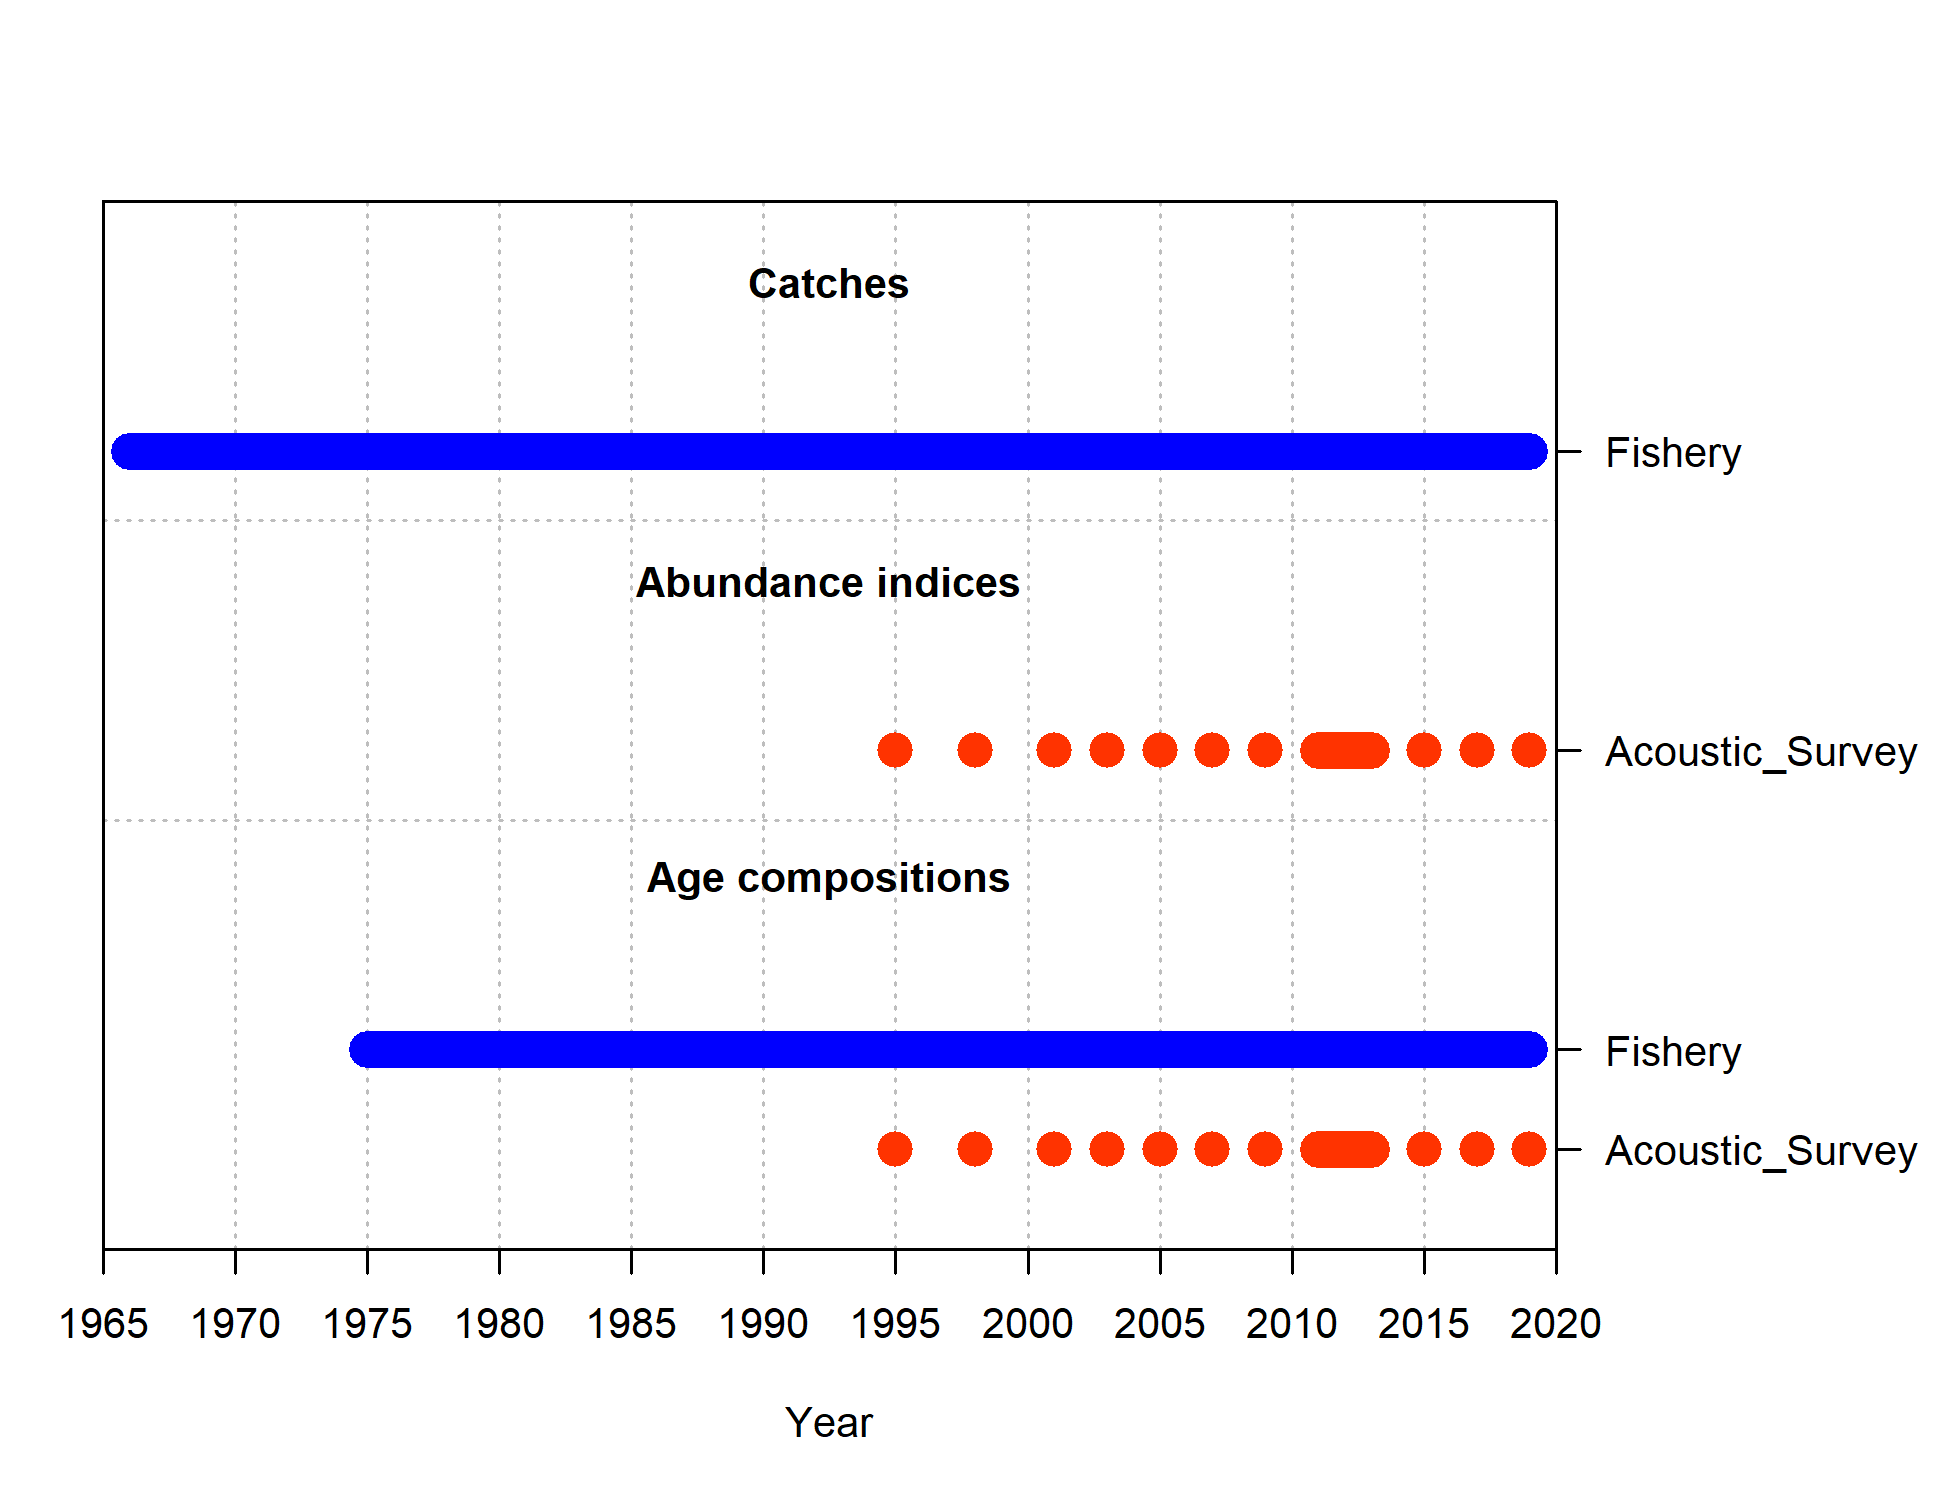
\includegraphics[width=1\textwidth,height=1\textheight]{data-plot.png}
\caption{Summary of data sources used in the base model.\label{fig:data-plot}}
\end{figure}

\tagmcend\tagstructend

\tagstructbegin{tag=Figure,alttext={Estimated time-series of total biomass.}}\tagmcbegin{tag=Figure}

\begin{figure}
\centering
\includegraphics[width=1\textwidth,height=1\textheight]{N://Assessments/CurrentAssessments/DataModerate_2021/copper_rockfish/models/wa/0.0_init_model/plots/ts1_Total_biomass_(mt).png}
\caption{Estimated time-series of total biomass for Copper Rockfish.\label{fig:total_bio}}
\end{figure}

\tagmcend\tagstructend

\tagstructbegin{tag=Figure,alttext={Test figure.}}\tagmcbegin{tag=Figure}

\begin{figure}
\centering
\includegraphics[width=1\textwidth,height=1\textheight]{N:/Assessments/CurrentAssessments/DataModerate_2021/copper_rockfish/models/wa/0.0_init_model/plots/ts7_Spawning_output.png}
\caption{Test figure.\label{fig:test}}
\end{figure}

\tagmcend\tagstructend

\clearpage

\tagstructbegin{tag=H1}\tagmcbegin{tag=H1}

\hypertarget{references}{%
\section{References}\label{references}}

\leavevmode\tagmcend\tagstructend

\hypertarget{refs}{}
\begin{cslreferences}
\leavevmode\hypertarget{ref-bradburn_2003_2011}{}%
Bradburn, M. J., A. A Keller, and B. H. Horness. 2011. ``The 2003 to 2008 US West Coast Bottom Trawl Surveys of Groundfish Resources Off Washington, Oregon, and California: Estimates of Distribution, Abundance, Length, and Age Composition.'' US Department of Commerce, National Oceanic; Atmospheric Administration, National Marine Fisheries Service.

\leavevmode\hypertarget{ref-hamel_method_2015}{}%
Hamel, Owen S. 2015. ``A Method for Calculating a Meta-Analytical Prior for the Natural Mortality Rate Using Multiple Life History Correlates.'' \emph{ICES Journal of Marine Science: Journal Du Conseil} 72 (1): 62--69. \url{https://doi.org/10.1093/icesjms/fsu131}.

\leavevmode\hypertarget{ref-weinberg_2001_2002}{}%
Weinberg, K. L., M. E. Wilkins, F. R. Shaw, and M. Zimmermann. 2002. ``The 2001 Pacific West Coast Bottom Trawl Survey of Groundfish Resources: Estimates of Distribution, Abundance and Length and Age Composition.'' NOAA Technical Memorandum NMFS-AFSC-128. U.S. Department of Commerce.
\end{cslreferences}
\end{document}
